\chapter{Motor Control and Communication}
\label{chap:mcc}

The \ac{MCC} subsystem is responsible for providing sufficient thrust to the airship for its movement and for providing communication with a controller on the ground.

\section{Functional and Technical Requirements}

\subsection{Functional Requirements}
%What function(s) does the subsystem have to fulfill?

Below are listed the primary functional requirements for the \ac{MCC}:

\begin{itemize}
\item Reliable communication between ground controller (transmitter) \& airship (receiver)
\item Independent speed control for each of the motors and provision of sufficient thrust to the airship
\item Operation of the airship from the ground 
\end{itemize}

\subsection{Technical Requirements}
%What technical requirements constrain the subsystem design? - e.g. mass, power, strength, stability etc.

The technical requirements for the \ac{MCC} subsystem are presented in Table \ref{tab:technical}.

\begin{table}[H]
\centering
\caption{Technical requirements}
\label{tab:technical}
\begin{tabular}{c c}
\hline
\textbf{Parameter} & \textbf{Value}\\ \hline
Total mass & $50\,g$\\
Input voltage & $3.8\,V$\\
Maximum power consumption & $50-60\,W$\\
Transmission frequency & $2.4\,GHz$\\
Receiver channels & $6$\\
Maximum cost & $2500\,SEK$\\
\hline
\end{tabular}
\end{table}

\noindent
As it was decided to use a blimp from ESRANGE instead of the custom-built \ac{MSE} (see chapter \ref{chap:mse}), the whole system had to be redesigned. The main changes were the increased dimensions of the blimp and the decreased total lift mass. This required for the\ac{MCC} to use more powerful and more efficient motors, since the \ac{EPS} was affected as well. The transmitter/receiver system however remained unchanged.

\subsection{Expected Performance}
%What are the expected performances of the subsystem, as related to the requirements above? (maybe including some margins)

\begin{itemize}
\item Motor efficiency: 77 \% 
\item RPM (for each motor): 1400 RPM/V
\end{itemize}

\section{Critical Design}
%Explain the preliminary design including block diagrams, schematics, drawings, etc.

The functioning of the \ac{MCC} subsystem is shown in Figure \ref{fig:design_block}. The transceiver consists of a 2.4 GHz transmitter and receiver (see below). The receiver forwards the motor speed control commands to the \ac{ESC} which in turn control the motor to reach the desired speed.

\begin{figure}[h!]
\centering
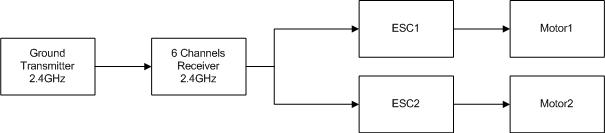
\includegraphics[scale=0.8]{figures/blockdiagram.jpg}
\caption{Block diagram}
\label{fig:design_block}
\end{figure}

\subsection{Motors}

Brush-less motors are selected as they are known to be powerful and light at the same time. The mass of the selected motors is $38\ g$, with dimensions of $27.6 \times 11 mm$ (see Figure \ref{fig:Motors}).

\begin{figure}[bht]
\centering
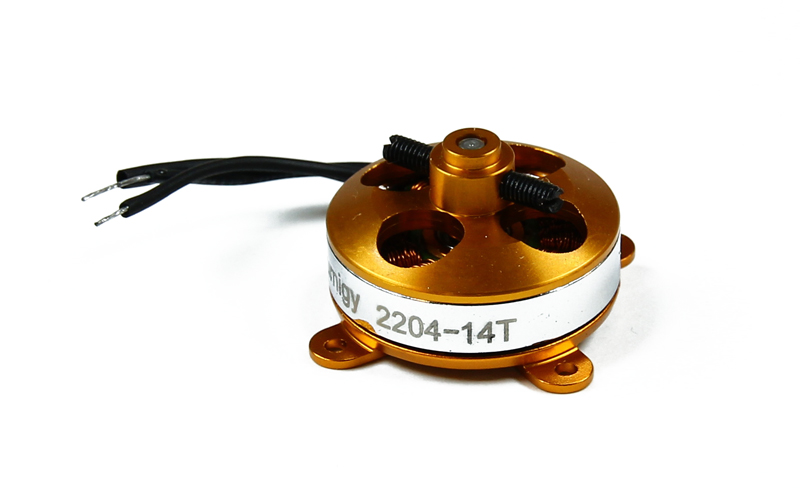
\includegraphics[scale=0.25]{figures/Motors.jpg}
\caption[Motors for the MCC]{Motors for the MCC \cite{website:rcflight}}
\label{fig:Motors}
\end{figure}

\noindent
The speed of the motor can be controlled by the following methods:

\begin{itemize}
\item Use a \ac{COTS} \ac{ESC} for each motor
\item Build a motor speed controller using a microprocessor
\end{itemize}

\noindent
The primary advantage of using \ac{COTS} \ac{ESC}s is the ease of use. This reduces the development cycle to a large extent. The disadvantage of using it is limited scalability i.e. functions like autonomous control and telemetry and telecommanding are not possible. Nevertheless, \ac{COTS} \ac{ESC}s will be used to control the speed of the motors because of time constraints. If time permits it will be desirable to build a speed controller with the help of a microprocessor. The new motors however require a higher current than the motors that were originally selected. Therefore suitable \ac{ESC}s are selected which are able to supply a maximum current of 10 $A$.

\subsection{Transceiver System}
%Which design concepts are considered? - What are the advantages/disadvantages for each concept?

For the transceiver system the available options are to use

\begin{itemize}
\item A 72 MHz transceiver system that uses Amplitude/Frequency Modulation
\item A 2.4 GHz transceiver system that uses Spread Spectrum Technology
\end{itemize}

\noindent
A comparison between these two technologies is shown in Table \ref{tab:transceiver}.

\begin{center}
\begin{table}[bht]
\caption{Transceiver systems}
\begin{tabular}{|l l l|}
\hline
\textbf{Parameter:} &  \textbf{2.4 GHz Transceiver} & \textbf{72 MHz Transceiver}\\ 
\hline
Frequency Used & 2.4 GHz & 72 MHz \\
Crystal Used & No & Yes \\
Change in Frequency & On next power up & By changing the crystal \\
Ability to transmit through obstacles & Weak & Very Good\\
Bandwidth & Wide & Narrow\\
Data Rate & High & Low\\
Power Usage & Less & More\\
RF Noise Immunity & Very Good & Less \\
\hline
\end{tabular}
\label{tab:transceiver}
\end{table}
\vspace{-2.0em}
\end{center}

\noindent
It is clear from Table \ref{tab:transceiver} that a 2.4 GHz transceiver system is better for the chosen application. The only disadvantage of using a 2.4 GHz transceiver system is that the receiver should have very reliable batteries and the voltage should constantly be maintained at a particular level. The reason is that there are small processors in the transmitter and receiver that carry out many complex calculations every second. These processors require a constant steady supply of current to work properly. If there is an interruption in the supply current of the receiver there will be problems with the communication channel.
\\
\\
The 2.4 GHz transceiver system is selected for the communication channel. The transceiver uses the 2.4 GHz frequency band and the spread spectrum technology for transmission of signals. This feature helps in removing all interfering frequencies caused by other electronic equipments which improves the communication channel. The other major advantage of using spread spectrum technology is that the communication channel is not affected, even when someone is using the same frequency band.

%\subsection{Telemetry and Telecommands}
%%What telemetries/telecommands are required/useful for the subsystem? – What data rates/sizes are required?
%
%If time permits, it would be desirable to have a microprocessor for telecommanding and telemetry  which is listed in Table \ref{tab:Telemetry}
%
%\begin{table}[h]
%\centering
%\begin{tabular}{|l|l|l|}
%\hline
%\textbf{Telemetry} & \textbf{Data rate/frequency} & \textbf{Data size} \\
%\hline
%Battery voltage & Every 30 sec & 1 byte \\
%\hline
%Solar array temperature & Every 30 sec & 1 byte\\
%\hline
%Solar array voltage & Every 1 sec(MPPT Performance) & 2 bytes\\
%\hline
%Solar array temperature & Every 1 sec ( MPPT Performance & 2 bytes\\
%\hline
%
%\end{tabular}
%\caption{Telemetry}
%\label{tab:Telemetry}
%\end{table}

